\subsection{Compact Convolutional Neural Network Accelerator for IoT Endpoint SoC}
\subsubsection{Khối tích chập}
\begin{figure}[!h]
    \centering
    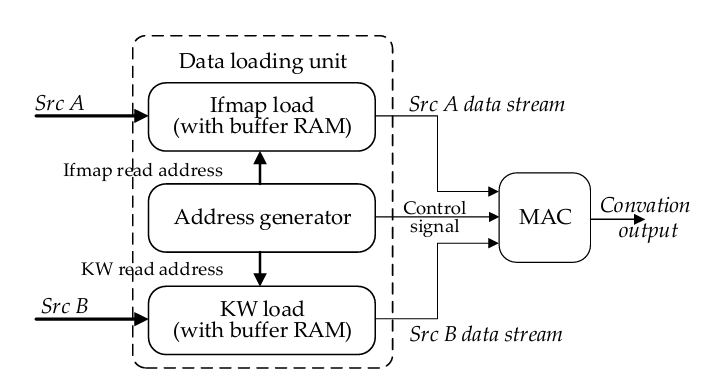
\includegraphics[width=0.5\textwidth]{Images/CNNAccelerator/CompactCNNAccelerator/conv_architecture.png}
    \vspace{10pt} % Thay đổi giá trị 10pt theo nhu cầu
    \caption{Kiến trúc của khối tích chập}
\end{figure}
Flow hoạt động của khối tích chập được thể hiện ở hình bên dưới:
\begin{figure}[!h]
    \centering
    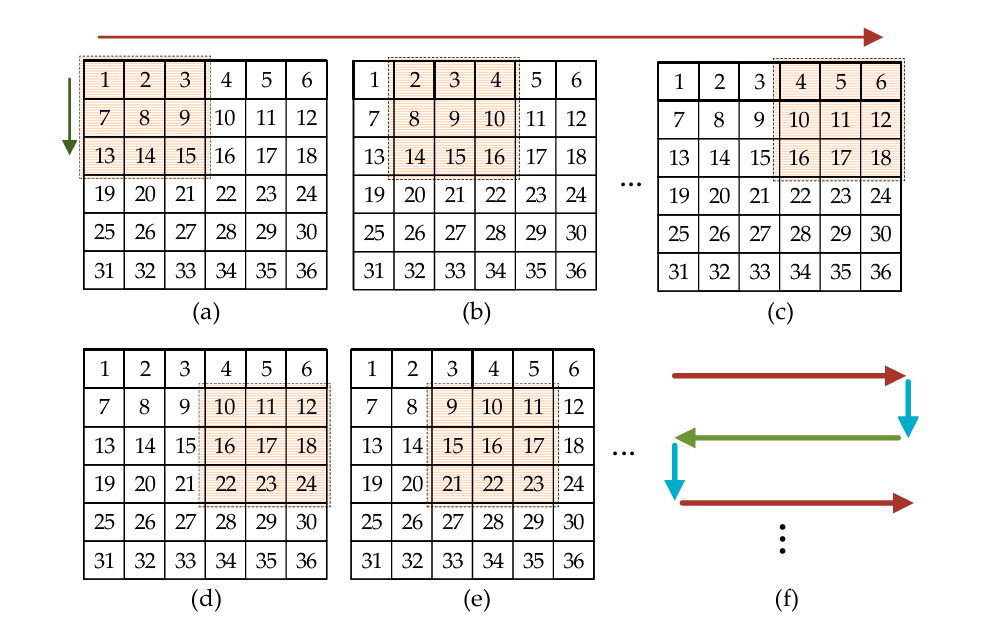
\includegraphics[width=0.7\textwidth]{Images/CNNAccelerator/CompactCNNAccelerator/conv_workflow.png}
    \vspace{10pt} % Thay đổi giá trị 10pt theo nhu cầu
    \caption{Workflow của khối tích chập}
\end{figure}

\begin{itemize}
    \item Đây là thành phần quan trọng nhất trong bộ gia tốc CNN vì CNN chủ yếu sử dụng phép toán tích chập. Thiết kế của đơn vị tích chập tập trung vào tối ưu hóa việc tải và lưu trữ dữ liệu.
    \item Sử dụng kỹ thuật giảm băng thông bộ nhớ bằng cách tận dụng sự lặp lại của dữ liệu trong phép toán tích chập, giúp giảm bớt băng thông cần thiết và tăng tốc độ tính toán.
    \item Các tín hiệu đầu vào được xử lý qua một bộ nhớ đệm (buffer RAM) để tối ưu hóa việc truy xuất dữ liệu.
\end{itemize}
\subsubsection{Khối Pooling}
Kiến trúc tổng quát của khối max-pooling được thể hiện ở sơ đồ bên dưới: 
\begin{figure}[!h]
    \centering
    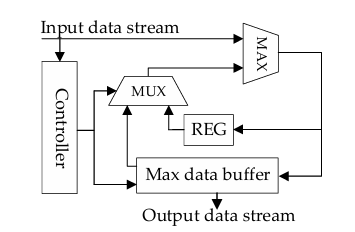
\includegraphics[width=0.5\textwidth]{Images/CNNAccelerator/CompactCNNAccelerator/pooling_architecture.png}
    \vspace{10pt} % Thay đổi giá trị 10pt theo nhu cầu
    \caption{Kiến trúc của khối pooling}
\end{figure}
\begin{itemize}
    \item Khối max-pooling thực hiện phương pháp max-pooling, giúp giảm kích thước dữ liệu đầu ra sau khi qua phép toán tích chập.
    \item Thiết kế của khối max-pooling là một mạch nối tiếp với bộ chọn và bộ so sánh (max comparator), cho phép giảm thiểu tài nguyên nhưng vẫn đảm bảo hiệu năng tính toán.
\end{itemize}
\subsubsection{Khối Multifunctional Accumulation Unit}
 Khối này được sử dụng để tích lũy kết quả của nhiều phép tích chập 2D. Nó cũng được chia sẻ với lớp bias, đơn giản hóa thiết kế và giảm tiêu thụ tài nguyên.
\subsubsection{Thiết kế chuỗi tăng tốc}
Chuỗi tăng tốc được thể hiện ở sơ đồ bên dưới:
\begin{figure}[!h]
    \centering
    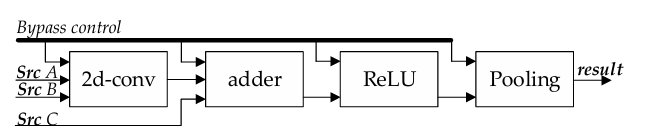
\includegraphics[width=0.5\textwidth]{Images/CNNAccelerator/CompactCNNAccelerator/chain_architecture.png}
    \vspace{10pt} % Thay đổi giá trị 10pt theo nhu cầu
    \caption{Kiến trúc của chuỗi tăng tốc}
\end{figure}
Bộ tăng tốc CNN được thiết kế theo dạng chuỗi gia tốc để tối ưu hóa hiệu suất tính toán. Mỗi chuỗi tăng tốc có thể thực hiện nhiều phép toán cùng lúc, giảm bớt sự di chuyển của dữ liệu giữa các phép toán và tăng hiệu suất tính toán. Cấu trúc của chuỗi tăng tốc bao gồm:
\begin{itemize}
    \item 4 chuỗi tăng tốc (acceleration chains): Mỗi chuỗi có thể thực hiện một phép toán tích chập độc lập, đồng thời giảm thiểu sự trùng lặp trong việc sử dụng tài nguyên.
    \item Kênh dữ liệu (Data Channels): Mỗi chuỗi gia tốc sử dụng các kênh dữ liệu như Src A, Src B, Src C, và kênh kết quả để chia sẻ thông tin giữa các thành phần khác nhau của bộ gia tốc.
\end{itemize}
Thiết kế này giúp xử lý song song nhiều lớp CNN với hiệu suất cao, đồng thời tiết kiệm tài nguyên bộ nhớ và giảm tiêu thụ năng lượng.\\
Bộ tăng tốc sử dụng một hệ thống điều khiển bypass để bỏ qua các module không cần thiết trong mỗi lớp mạng CNN, nhằm tối ưu hóa tốc độ xử lý. Các phép toán cũng được điều chỉnh độ rộng dữ liệu để phù hợp với kiến trúc 10-bit fixed-point, điều này giúp tiết kiệm tài nguyên mà không ảnh hưởng lớn đến độ chính xác. Bảng bên dưới cho thấy ảnh hưởng của độ rộng dữ liệu đối với độ chính xác của thuật toán là không đáng kể.
\subsubsection{Kiến trúc bộ tăng tốc}
Kiến trúc tổng quát của bộ tăng tốc được thể hiện ở sơ đồ bên dưới:
\begin{figure}[!h]
    \centering
    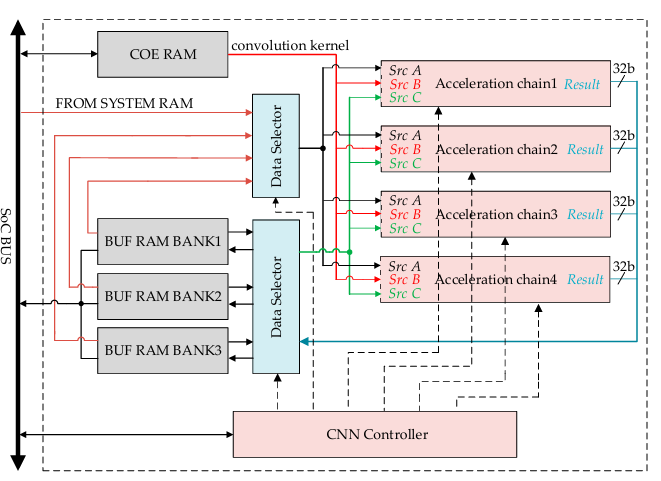
\includegraphics[width=0.7\textwidth]{Images/CNNAccelerator/CompactCNNAccelerator/accelerator_architecture.png}
    \vspace{10pt} % Thay đổi giá trị 10pt theo nhu cầu
    \caption{Kiến trúc của bộ tăng tốc}
\end{figure}
\begin{itemize}
    \item Bộ tăng tốc bao gồm bộ điều khiển CNN, ba khối đệm, bốn chuỗi tăng tốc và bộ chọn dữ liệu.
    \item Kiến trúc cho phép bộ tăng tốc thực hiện đồng thời các phép tích chập, kích hoạt và lấy mẫu con với bốn nhân tích chập dựa trên việc sử dụng ma trận nguồn, tăng hiệu suất tính toán.
    \item Bộ nhớ BUF RAM BANK được sử dụng để lưu trữ psum, ma trận nguồn và kết quả đệm, giảm thiểu việc di chuyển dữ liệu và tăng hiệu suất hệ thống. Mỗi BUF RAM BANK được ghép nối từ bốn SP-RAM độc lập để tăng băng thông truy cập.
    \item Bảng bên dưới tóm tắt các thông số cơ bản của bộ tăng tốc, cho thấy nó có thể đáp ứng các yêu cầu nhận dạng hình ảnh chung của SoC đầu cuối IoT.
\end{itemize}
\subsubsection{Thực nghiệm}
Để kiểm tra tính khả thi và hiệu quả của bộ gia tốc thiết kế, nhóm tác giả đã thực hiện một loạt thử nghiệm trên nền tảng FPGA, mô phỏng một hệ thống SoC (System-on-Chip) với bộ xử lý Cortex-M3.\\
Nền tảng thử nghiệm sử dụng vi xử lý ARM Cortex-M3 và chạy mạng Lenet-5 làm ví dụ.. Các thành phần chính của nền tảng thử nghiệm bao gồm:
\begin{itemize}
    \item Nền tảng được xây dựng dựa trên lõi Cortex-M3, một lõi MCU phổ biến của ARM cung cấp sự cân bằng tốt giữa hiệu suất và mức tiêu thụ năng lượng.
    \item SoC thử nghiệm bao gồm 128 KB RAM, 128 KB ROM và các thiết bị ngoại vi thông thường như GPIO và UART.
    \item SoC sử dụng bus AHB và APB để kết nối các thiết bị với lõi, với các thiết bị tốc độ cao như SCCB và bộ tăng tốc CNN được kết nối thông qua bus AHB, trong khi các thiết bị tốc độ thấp như GPIO được kết nối thông qua bus APB.
    \item Bảng dưới cho thấy mức tiêu thụ tài nguyên LUT của SoC khi được tổng hợp và triển khai trên FPGA. Bộ tăng tốc CNN chiếm 4901 LUT, chiếm tỷ lệ đáng kể trong tổng mức tiêu thụ tài nguyên của SoC.
\end{itemize}
Triển khai mạng kiểm thử Lenet-5
\begin{itemize}
    \item Mạng Lenet-5 được sử dụng để đánh giá bộ tăng tốc CNN. Lenet-5 là một mạng CNN cổ điển với các lớp tích chập (convolution layers), lớp gộp (subsampling), và lớp kết nối đầy đủ (fully connected). Việc triển khai mạng Lenet-5 trên nền tảng thử nghiệm giúp kiểm tra khả năng của bộ gia tốc trong việc xử lý các tác vụ nhận diện hình ảnh.
\end{itemize}
Kết quả thực nghiệm:
\begin{itemize}
    \item Hiệu suất của bộ tăng tốc được so sánh với CPU Intel i5 7500 và hai bộ xử lý ứng dụng di động Samsung S5P6818 và AllWinner H3
    \item Thời gian thực thi của Lenet-5 được đo trên các nền tảng khác nhau và được hiển thị ở bên dưới:
    \begin{figure}[!h]
    \centering
    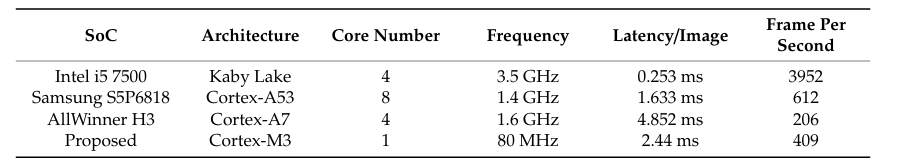
\includegraphics[width=\textwidth]{Images/CNNAccelerator/CompactCNNAccelerator/performance_table.png}
    \vspace{10pt} % Thay đổi giá trị 10pt theo nhu cầu
    \caption{Hiệu năng}
\end{figure}
\end{itemize}
Mức tiêu thụ tài nguyên:
Bài báo so sánh mức tiêu thụ tài nguyên của bộ tăng tốc được đề xuất với các bộ tăng tốc khác được báo cáo trong các tài liệu tham khảo:
\begin{itemize}
    \item Zhang, Y.; Wu, N.; Zhou, F.; Yahya, M.R. Design of Multifunctional Convolutional Neural Network Accelerator for IoT Endpoint SoC. In Proceedings of the World Congress on Engineering and Computer Science 2018, San Francisco, CA, USA, 23–25 October 2018; pp. 16–19.
    \item  Li, Z.; Wang, L.; Guo, S.; Deng, Y.; Dou, Q.; Zhou, H.; Lu, W. Laius: An 8-bit fixed-point CNN hardware inference engine. In Proceedings of the 2017 IEEE International Symposium on Parallel and Distributed Processing with Applications and 2017 IEEE International Conference on Ubiquitous Computing and Communications (ISPA/IUCC), Guangzhou, China, 12–15 December 2017; pp. 143–150.
    \item  Guo,K.; Sui, L.; Qiu, J.; Yu, J.; Wang, J.; Yao, S.; Han, S.; Wang, Y.; Yang, H. Angel-Eye: A complete design flow for mapping CNN onto embedded FPGA. IEEETrans. Comput. Des. Integr. Circuits Syst. 2018, 37, 35–47.
\end{itemize}
Kết quả được hiển thị ở bảng bên dưới:
\begin{figure}[!h]
    \centering
    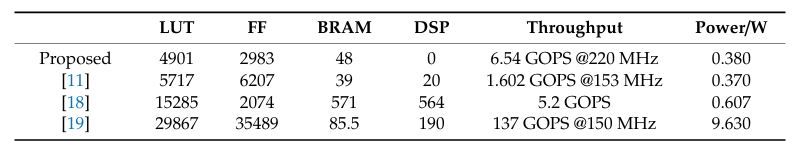
\includegraphics[width=0.7\textwidth]{Images/CNNAccelerator/CompactCNNAccelerator/resource_consumption_table.png}
    \vspace{10pt} % Thay đổi giá trị 10pt theo nhu cầu
    \caption{Mức tiêu thụ tài nguyên}
\end{figure}




